\documentclass[9pt]{beamer}
\mode<presentation>

% Theme choice:
\usetheme{Madrid}%Darmstadt 

\usecolortheme[RGB={0,100,50}]{structure}
 \usefonttheme{structurebold} 
\setbeamercovered{invisible}
%\setbeamertemplate{navigation symbols}{}
\usepackage{dynblocks}
\usepackage{textpos}
\usepackage{amsfonts}
\usepackage{amsmath}
\usepackage{amssymb}
\usepackage{amsthm}
\usepackage{dsfont}
\usepackage{mathtools}
\usepackage{dutchcal}
\usepackage{hyperref}
\usepackage[utf8]{inputenc}
\usepackage[T1]{fontenc}
\usepackage{listings}
\usepackage{xcolor}

\definecolor{codegreen}{rgb}{0,0.6,0}
\definecolor{codegray}{rgb}{0.5,0.5,0.5}
\definecolor{codepurple}{rgb}{0.58,0,0.82}
\definecolor{backcolour}{rgb}{0.95,0.95,0.92}

\lstdefinestyle{mystyle}{
    backgroundcolor=\color{backcolour},   
    commentstyle=\color{codegreen},
    keywordstyle=\color{magenta},
    numberstyle=\tiny\color{codegray},
    stringstyle=\color{codepurple},
    basicstyle=\ttfamily\footnotesize,
    breakatwhitespace=false,         
    breaklines=true,                 
    captionpos=b,                    
    keepspaces=true,                 
    numbers=left,                    
    numbersep=5pt,                  
    showspaces=false,                
    showstringspaces=false,
    showtabs=false,                  
    tabsize=2
}

\lstset{style=mystyle}

\hypersetup{
    colorlinks=true,
    linkcolor=blue,
    filecolor=magenta,      
    urlcolor=cyan,
    pdftitle={Overleaf Example},
    pdfpagemode=FullScreen,
    }

% Title page details: 
\title[Informatika]{GS Informatika} %add title


\author[]{ \textbf{\Large Daniel Rod}} %Add author
\date{Jazyk C}

% Logo only on title page
\usepackage[pscoord]{eso-pic}


\begin{document}

% Title page frame
%\begin{frame}
    %\titlepage 
%\end{frame}
\frame[plain]{\titlepage}
%logo
\AddToShipoutPictureFG{
    \put(\LenToUnit{.92\paperwidth},
    \LenToUnit{.185\paperheight})
    {\vtop{{\null}}}}


\begin{frame}{Outline}
  \tableofcontents
\end{frame}

\section{O jazyku C}

\begin{frame}{Programování v C}

\begin{block}{Jazyk C}
\begin{itemize}
    \item Low až Medium level jazyk
    \item Programování systémů (OS, embedded)
    \item Explicitní práce s pamětí
    \item ALGOL rodina jazyků
\end{itemize}
\end{block}

\pause

\begin{block}{Kompilace}
\begin{itemize}
    \item Běžné jsou kompilované implementace
    \item Před spuštěním jej musíme převést
    do spustitelného souboru
    \item Velmi starý model kompilace - často vyžaduje explicitní deklarace a implementace
    \item Využití textových souborů pro psaní kódu
\end{itemize}
\end{block}

\end{frame}

\begin{frame}{Programování v C}

\begin{block}{Typy souborů}
\begin{itemize}
    \item Hlavičkové soubory - běžně obsahují definice, přípona \textbf{.h}
    \item Zdrojové soubory - obsahují implementace, přípona \textbf{.c}
    \item Hlavičkové soubory nejsou nutností, hodí se ale pro
    \begin{itemize}
        \item Organizaci
        \item Modularitu
        \item "Reusability"
    \end{itemize}
\end{itemize}
\end{block}

\pause

\begin{block}{Definice a implementace}
    \begin{itemize}
        \item Definice nám pouze říká co funkce zkonzumuje za datové typy
        a co nám za datový typ vrátí
        \item Pro malé programy stačí jen jeden zdrojový soubor, nemusíme nutně separovat implementaci a definice
        \item Starší kompilery mohou být hloupé - definice by měla předcházet použití (to jsme v BSL/ISL neměli!)
    \end{itemize}
\end{block}

\end{frame}

\begin{frame}{Definice a implementace}
    \begin{center}
        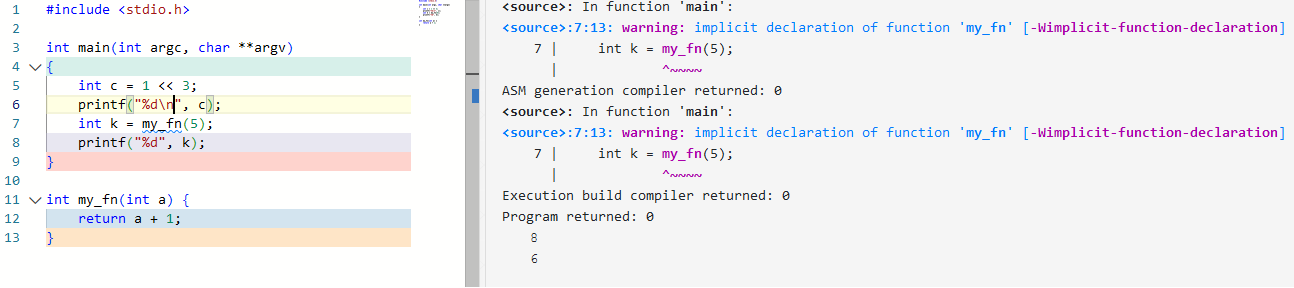
\includegraphics[width=0.98\linewidth]{lekce19/warning-implicit-fn-decl.png}
    \end{center}
\end{frame}

\begin{frame}{Programování v C}

    \begin{block}{Syntax jazyka}
    \begin{itemize}
        \item Jazyk C je procedurální - námi požadované operace se postupně provádějí, funkce jsou pak sady požadovaných operací
        \item Přiřazení hodnoty do proměnné je také operace!
        \item Validní identifikátory jsou omezenější oproti LISP/SCHEME dialektům
        \item Každá instrukce končí středníkem \textbf{;}
        \item Kód je dělen na bloky instrukcí
    \end{itemize}
    \end{block}
    
    \pause
    
    \begin{block}{Program}
        \begin{itemize}
            \item Každá program musí mít alespoň jednu funkci \textbf{main()}
            \item Při spuštění programu se provádí operace z funkce \textbf{main()}
        \end{itemize}
    \end{block}
\end{frame}

\begin{frame}{Jednoduchý program v C}

\begin{block}{První program}
\begin{itemize}
    \item Jednoduchý program který po spuštění vypíše \textit{Program v jazyce C}, odřádkuje a ukončí se
\end{itemize}
\end{block}

\pause

\lstinputlisting[language=C]{lekce19/program01.c}

\pause

\begin{block}{Kompilace}
    \begin{itemize}
        \item Zdrojový soubor je nejprve zkompilován do tzv. objektového souboru (\textit{s příponou} \textbf{.o}), kde se nachází \textit{relativní adresy} na proměnné, volání funkcí a reference na funkce bez známé implementace\
    \end{itemize}
\end{block} 
\end{frame}

\begin{frame}{Kompilace}
    \begin{block}{Od zdrojového souboru ke spustitelnému}
        \begin{itemize}
            \item Zdrojový soubor \textit{program01.c} je zkompilován pomocí kompilátoru (např. clang nebo gcc) \\
            \begin{center}
                \textbf{gcc program01.c}
            \end{center}
            \item To vytvoří nejprve objektový soubor, který následně převede na spustitelný soubor. Běžně nelze očekávat, že spustitelný soubor zkompilovaný na jednom počítači bude fungovat na jiném!
        \end{itemize}
    \end{block}
\end{frame}

\section{Hardware a principy počítačů}

\begin{frame}{Paměť a procesor}
    \begin{block}{Zjednodušené schéma - Harvardská architektura}
        \begin{center}
            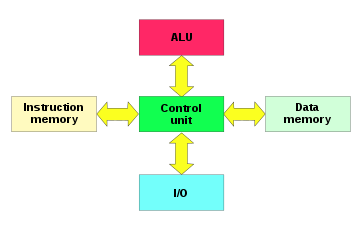
\includegraphics[width=0.8\linewidth]{lekce19/harvard-architecture.png}
        \end{center}
        (ALU se dá brát jako součást Control Unit spolu s registry a countery)
    \end{block}
\end{frame}

\begin{frame}{Paměť}
    \begin{block}{Paměťový adresový prostor}
        \begin{itemize}
            \item Data v paměti mají určitou lokaci - adresu
            \item Pokud používáme větší paměť (Instruction + Data), je třeba dostatečně velký adresový prostor \item Pro adresy o velikosti 32 bitů máme ~ 4GB paměti které můžeme adresovat (x86)
            \item 64bitové procesory - používají datové jednotky co mají až 64 bitů - máme "k dispozici" adresy přesahující velikosti dnešních RAM
        \end{itemize}
    \end{block}
    \pause
    \begin{block}{RAM}
    \begin{itemize}
        \item Random access memory - přistupujeme k libovolné hodnotě stejně rychle jako ke každé jiné (přibližně!)
        \item Bývá \textbf{volatile} - po vypnutí ztratí data
    \end{itemize}
    \end{block}
\end{frame}

\begin{frame}{Typy RAM}
    \begin{block}{SRAM}
    \begin{itemize}
        \item Static RAM
        \item Malá kapacita dat
        \item Rychlé - zejména sekvenční přístupy
    \end{itemize}
    \end{block}
    \pause
    \begin{block}{DRAM}
        \begin{itemize}
            \item Dynamic RAM
            \item Levnější a větší (řádově GB)
            \item Pomalejší
        \end{itemize}
    \end{block}
\end{frame}

\begin{frame}{Slovo (WORD) a instrukce}
    \begin{block}{WORD - jednotka velikosti}
        \begin{itemize}
            \item Udává "jednotku přenosu" dat
            \item n-bitové zařízené - slovo má velikost n bitů
            \item Instrukce pracují s daty o velikosti slov
            \item Historicky - ve starém kódu se můžeme setkat s DWORD - 32b
            \item V x86 má například WORD 32b a adress space je 32b
        \end{itemize}
    \end{block}
    \pause
    \begin{block}{Instrukce}
        \begin{itemize}
            \item Posloupnost n bytů
            \item Instrukční sada - které instrukce umí procesor (např. \href{https://en.wikipedia.org/wiki/X86_instruction_listings}{základní známe x86 instrukce})
            \item Strojový kód - posloupnost instrukcí
            \item Instruction Pointer - pozice momentálně vykonávané instrukce (pokud je vícebytová typicky ukazuje na první byte)
            \item Zpravidla má stejnou velikost jako bloky code memory
            \item Opcode - typ instrukce, následují jej argumenty (adresy)
        \end{itemize}
    \end{block}
\end{frame}

\begin{frame}{Příznakový registr CPU}
\begin{block}{Vlajky(flags)}
    \begin{itemize}
        \item flag je 1 bit informace (Ano / Ne)
        \item Příznakový registr pomocí flags uchovává
        informace o probíhajících výpočtech
        \item Ne všechny instrukce se dokončí v jednom \textit{cyklu}
        \item Sčítání zabere 1-2 cykly (2 v případě velkých čísel, používá se carry flag - přenos z výsledku v předchozím cyklu a sign flag - jestli vyšel předchozí cyklus záporně)
        \item Násobení 32 bit čísel - 10 cyklů + carry flag + sign flag
        \item Násobení 64 bit čísel - 20 cyklů + carry flag + sign flag
        \item Dělení 32 bit čísel - 70 cyklů!
        
    \end{itemize}
\end{block}
    
\end{frame}

\begin{frame}{Assembler}
    \begin{block}{Instrukce čitelně}
        \begin{itemize}
            \item Instrukce jsou posloupnost bytů (reprezentujeme dvojice jako HEX cifry) - špatně se čtou
            \item Assembler přiřazuje opcodes jména
        \end{itemize}
    \end{block}

    \begin{center}
        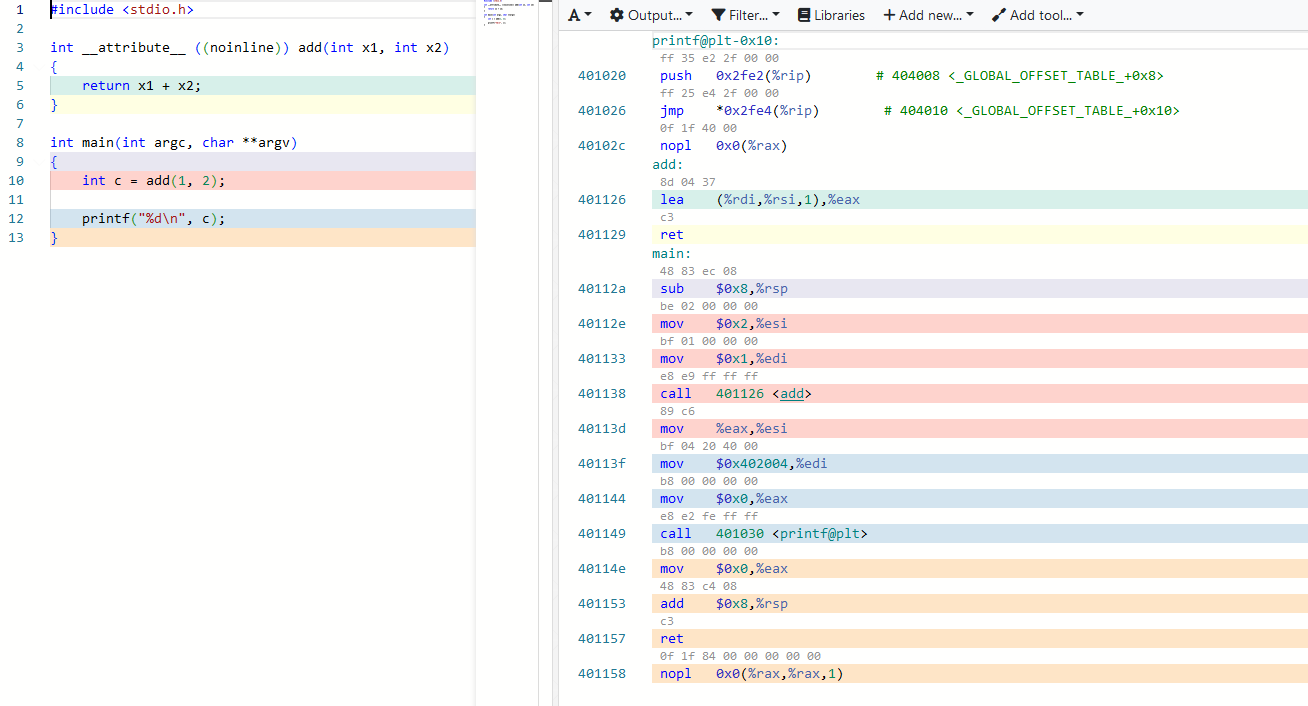
\includegraphics[width=0.9\linewidth]{lekce19/assembler.png}
    \end{center}
\end{frame}

\section{Kompilace programu v C (podrobněji)}
\begin{frame}{Kompiler - součásti}
    \begin{block}{Preprocessor}
        \begin{itemize}
            \item Překlad maker - příkazy s prefixem \textbf{\#}
            \item Vlastní makra - nahrazování "textu za text"
            \item Makra mohou mít argumenty
        \end{itemize}
    \end{block}
    \pause
    \begin{block}{Kompilátor}
        \begin{itemize}
            \item V několika "passech" projede jednotlivé zdrojové soubory a vytvoří objektové soubory.
            \item Překládá námi napsané příkazy na instrukce
            \item Pracuje se soubory separátně - proto potřebujeme hlavičkové soubory! Soubour prg1.c neví nic o implementaci funkce z prg2.c, jen víme že je deklarovaná v prg2.c
        \end{itemize}
    \end{block}
    \pause
    \begin{block}{Linker}
         \begin{itemize}
             \item Propojí jednotlivé objektové soubory - pokud volám z prg1.c funkci v prg2.c, až po projetí linkerem bude toto volání "funkční"
             \item Zajistí přiřazení objektových souborů referencovaných knihoven (BSL/ISL require)
         \end{itemize}
    \end{block}
\end{frame}

\section{Jazyk C - základy}

\begin{frame}{Základní datové typy}
    \begin{block}{Číselné datové typy}
        \begin{itemize}
            \item Ze začátku budeme pracovat zejména s čísly
            \item C je striktně typovaný - každá proměnná musí mít deklarovaný typ
            \item signed / unsigned typy - určuje jestli mají "znaménko", signed je default
            \item Velikost v paměti \textbf{závisí na implementaci}! Zjistíme pomocí \textit{sizeof(T)}
        \end{itemize}
    \end{block}

    \begin{block}{Celá čísla}
        \begin{itemize}
            \item \textbf{short}
            \item \textbf{int}
            \item \textbf{long}
            \item \textbf{long long}
        \end{itemize}
    \end{block}

    \begin{block}{Desetinná čísla}
        \begin{itemize}
            \item \textbf{float}
            \item \textbf{double}
            \item \textbf{long double}
        \end{itemize}
    \end{block}
\end{frame}

\begin{frame}{Základní datové typy}
    \begin{block}{Dodatek - char}
        \begin{itemize}
            \item Char je nejmenší číselný typ, běžně se ale používá pro \textbf{ukládání textu} (jako 1-String)
        \end{itemize}
    \end{block}

    \begin{block}{Speciální typy}
        \begin{itemize}
            \item size\_t - unsigned typ běžně používaný pro "velikost" - hodnoty mají max velikost odpovídající maximální velikosti "objektů"
            \item intptr\_t - (\textit{\#include <stdint.h>}) unsigned typ do kterého lze uložit validní pointery, používá se při pointer aritmetice (bude nás zajmat až později) 
        \end{itemize}
    \end{block}    
\end{frame}

\begin{frame}{Ukázka C programu}
    \lstinputlisting[language=C]{lekce19/program02.c}
\end{frame}

\begin{frame}{Deklarace a definice funkce}
    \begin{block}{Deklarace}
    \begin{itemize}
        \item Deklarace obsahuje jen hlavičku funkce - jméno funkce, jaké parametry (a jakého typu) funkce má a jaký typ proměnné vrací
        \item Deklarace nejsou povinné, je ale vhodné funkce deklarovat před použitím (při čtení kódu "od shora")
    \end{itemize}
    \end{block}
    \lstinputlisting[language=C]{lekce19/deklarace.c}
    \pause
    \begin{block}{Definice}
        \begin{itemize}
            \item Zavádí implementaci funkce - říká, jak funkce procedurálně postupuje a jak dosáhne výsledku který může vrátit
            \item Uvnitř funkce máme implicitně local prostředí - můžeme zavádět proměnné, které budou "existovat" jen v rámci
            běhu funkce
            \item Nelze mít "funkci ve funkci"
        \end{itemize}
    \end{block}
\end{frame}

\begin{frame}{Deklarace a definice funkce}
    \lstinputlisting[language=C]{lekce19/implementace.c}
    \pause
    \begin{block}{Funkce co nic nevrací}
        \begin{itemize}
            \item V některých případech chceme, aby funkce nic nevracela
            \item Návratový "typ" \textbf{void} - funkce nevrací žádnou hodnotu (void znamená "žádný typ")
            \item Např. při vypisování
        \end{itemize}
    \end{block}
    \lstinputlisting[language=C]{lekce19/void_implementace.c}
\end{frame}

\begin{frame}{Celý program}
\begin{center}
    DEMO
\end{center}
\end{frame}

\begin{frame}{Proměnné}
    \begin{block}{Deklarace}
        \begin{itemize}
            \item Proměnné můžeme nejprve deklarovat, kompiler pak ví že má vyhradit místo v paměti pro tuto proměnnou
            \item Deklarovaná proměnná má tedy \textit{adresu}, ale nemá "explicitní" hodnotu.
        \end{itemize}
        \begin{center}
            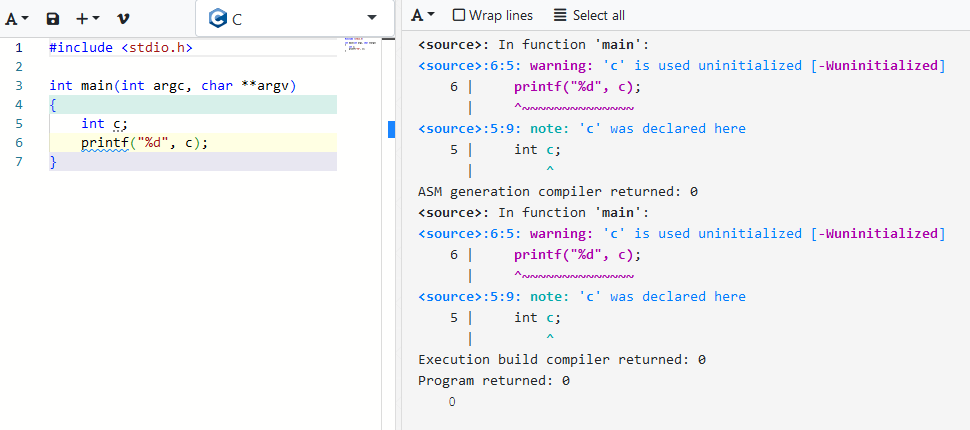
\includegraphics[width=0.8\linewidth]{lekce19/unassigned.png}
        \end{center}
    \end{block}
\end{frame}

\begin{frame}{Proměnné}
    \begin{block}{Přiřazení (assignment) a mutace / reassignment}
        \begin{itemize}
            \item Deklarované proměnné můžeme přiřadit hodnotu (nebo provést zároveň deklaraci a přiřazení)
            \item Do paměti vyhrazené pro proměnnou se uloží data
            \item Proměnná je v C tzv. l-value -> má pevně stanovenou adresu!
            \item Data na této adrese můžeme upravit -> měníme hodnotu proměnné!
        \end{itemize}
    \end{block}
    \lstinputlisting[language=C]{lekce19/promenne.c}
\end{frame}

\begin{frame}{l-values a r-values}
    \begin{block}{l-value}
        \begin{itemize}
            \item Výraz který se po vyhodnocení odkazuje na \textbf{paměť}
            \item Může být na levé i pravé straně přiřazovacího operátoru =
        \end{itemize}
    \end{block}
    \begin{block}{r-value}
        \begin{itemize}
            \item Výraz který se neodkazuje na žádnou adresu
            \item Jen na pravé straně přiřazovacího operátoru =
            \item Např. konstanta
        \end{itemize}
    \end{block}
\end{frame}

\begin{frame}{Komentáře v kódu}
    \begin{block}{Komentáře}
        \begin{itemize}
            \item Hlavička funkce obsahuje informace o typech
            \item Stále je vhodné popsat co funkce dělá, případně jak
            \item Řádkové komentáře pomocí //
            \item Komentáře pomocí /*   */
        \end{itemize}
    \end{block}
    \lstinputlisting[language=C]{lekce20/comment.c}
\end{frame}

\begin{frame}{Cvičení}
    \begin{block}{Funkce a proměnné}
    Cílem je spočítat počet zrnek kávy na šachovnici podle následujícího vzoru:
    Na prvním čtverci je 1 zrnko, na druhém 2, na každém dalším pak dvojnásobek.
    \begin{enumerate}
        \item Deklarujt proměnnou \textit{square\_count} typu \textit{int} v globálním scope.
        \item Deklarujte funkci \textit{square\_grains} s návratovým typem \textit{int} a jedním argumentem \textit{square\_number} typu \textit{int}, funkci zatím neimplementujte.
        \item Deklarujte funkci \textit{total\_grains} s návratovým typem \textit{int} a jedním argumentem \textit{total\_squares} typu \textit{int}, funkci zatím neimplementujte.
        \item Implementujte funkci main, která spočítá počet zrnek na šachovnici s počtem polí \textit{square\_count} a výpíše tento počet. Funkce main následně vrátí hodnotu \textit{"success"} - číslo 0. (Hint: pro vypsání použíjte funkci \textit{printf("\%d\textbackslash{}n", ...);} z knihovny \textit{stdio})
    \end{enumerate}
    Náš program zatím nejde zkompilovat, ale je korektní - implementace funkcí by totiž mohla klidně být v jiném zdrojovém souboru - chybu dostaneme až při kompilaci, kdy implementaci neposkytneme!
    Pojďme trochu prozkoumat naše data
    \begin{enumerate}
        \item Kolik polí má typická šachovnice? Upravte podle této znalosti typy proměnných a argumentů funkcí. (Hint: \textit{int} je pro naše účely zbytečně "velký")
        \item Nalezněte v kódu alespoň jednu l-value a dvě r-value.
    \end{enumerate}
    \end{block}
\end{frame}

\begin{frame}{Poznámka - extern}
\begin{block}{Viditelnost a klíčové slovo extern}
    Když deklarujeme funkci (jako třeba v předchozím cvičení), C automaticky
    přidává klíčové slovo \textit{extern}, které kompileru říká, že může implementaci
    najít jinde. Až linker nás zastaví a vyhodí chybu pokud takto deklarovanou funkci
    nenajde v žádných knihovnách použitých při kompilaci.

    Modifikátor extern lze použít i na proměnné, tomu se ale zatím věnovat nebudeme.
\end{block}
\end{frame}

\section{Kontrolní struktury, pole}

\begin{frame}{Kontrolní struktury}
    \begin{block}{Rozhodování - if}
        \begin{itemize}
            \item Při běhu programu je třeba rozhodovat o hodnotách a podle toho vyhodnocovat různé větve logiky. K tomu může sloužit klíčové slovo \textit{if}.
        \end{itemize}
    \end{block}
    \lstinputlisting[language=C]{lekce20/control_structures01.c}
    \begin{block}{Rozhodněte}
        Co bude na výstupu tohoto kódu?
    \end{block}
\end{frame}

\begin{frame}{Kontrolní struktury}
    \begin{block}{Rozhodování - else}
        \begin{itemize}
            \item Kód se často větví na dvě možnosti, pak můžeme použít "if-else" přístup
        \end{itemize}
    \end{block}
    \lstinputlisting[language=C]{lekce20/control_structures02.c}
\end{frame}

\begin{frame}{Kontrolní struktury}
    \begin{block}{Early return}
        \begin{itemize}
            \item Pokud je to ale možné, je vhodnější tzv. early return přístup
            \item Rozhodování je separováno do samostatné funkce, nepoužíváme else
            ale při splnění podmínky rovnou vracíme
            \item Kód je pak více "lineární pro oči"
        \end{itemize}
    \end{block}
    \lstinputlisting[language=C]{lekce20/control_structures03.c}
\end{frame}

\begin{frame}{Kontrolní struktury}
    \begin{block}{Rozhodování - else if}
        \begin{itemize}
            \item Pokud potřebujeme rozlišit mezi několika možnostmi které se vylučují, lze použít \textit{else if} strukturu
            \item Opět většinou lze nahradit early returnem
        \end{itemize}
    \end{block}
    \lstinputlisting[language=C]{lekce20/control_structures04.c}
\end{frame}

\begin{frame}{Kontrolní struktury}
    \begin{block}{Rozhodování - switch}
        \begin{itemize}
            \item Pokud rozhodování zakládáme na nějáké hodnotě integer nebo char hodnoty, je možné použít switch statement
            \item Často se přeloží do ASM jinak než if-else if-else bloky (jumptables - efektivnější)
        \end{itemize}
    \end{block}
    \lstinputlisting[language=C]{lekce20/control_structures05.c}
\end{frame}

\begin{frame}{Kontrolní struktury}
    \begin{block}{Smyčky (loops)}
        \begin{itemize}
            \item Pro potřeby opakování nějákého algoritmu používáme smyčky for a while
        \end{itemize}
    \end{block}
    \begin{center}
    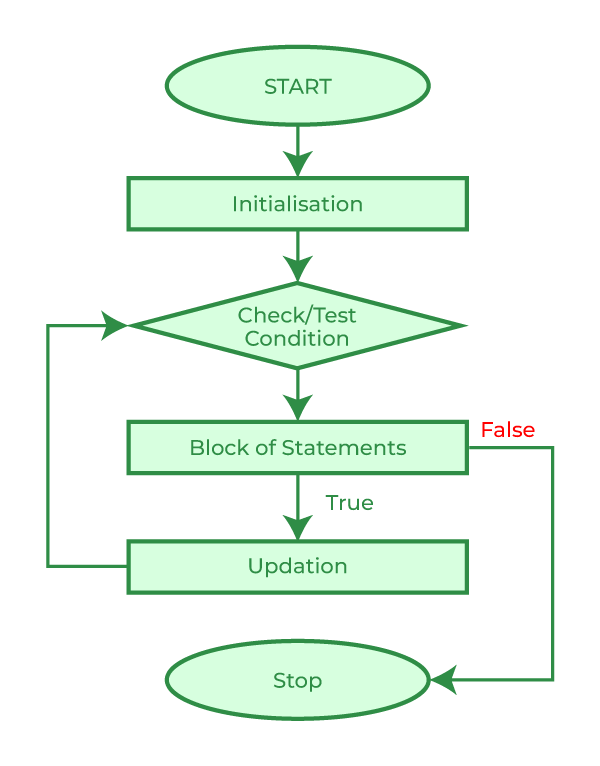
\includegraphics[width=0.35\linewidth]{lekce20/for_loop.png}
    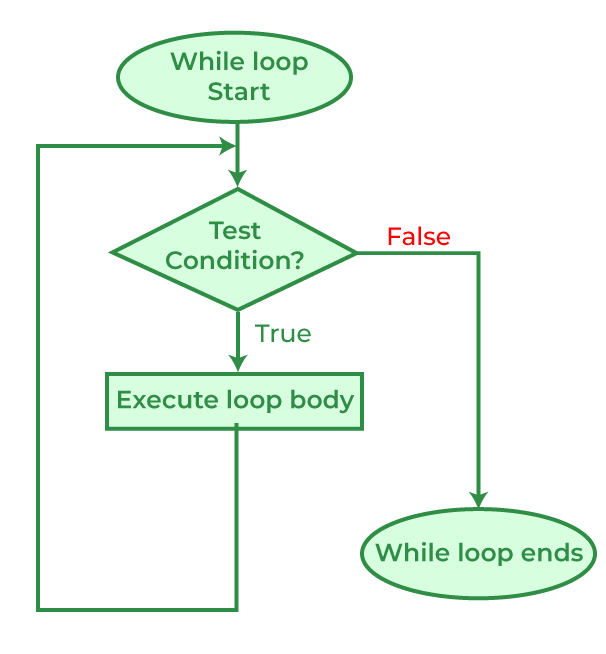
\includegraphics[width=0.35\linewidth]{lekce20/while_loop.png}
\end{center}
\end{frame}

\begin{frame}{Kontrolní struktury}
    \lstinputlisting[language=C]{lekce20/control_structures06.c}
\end{frame}

\begin{frame}{Procvičování - pokračování}
    \begin{block}{Funkce a proměnné}
    Implementujte funkce z předchozího cvičení (\textit{square\_grains} a \textit{total\_grains}).
    \begin{enumerate}
        \item Určete jak musí jednotlivé funkce "postupovat"
        \item Pomocí kontrolní struktur proveďte implementaci těchto postupů a otestujte
        \item Výpočet lze zjednodušit použitím správných matematických funkcí. O jaké funkce se jedná? Nalezněte je v C/C++ \href{https://en.cppreference.com}{referenci}
    \end{enumerate}
    \end{block}
\end{frame}

\begin{frame}{Pole}
    \begin{block}{Více dat v jedné proměnné}
        \begin{itemize}
            \item Stejně jako v BSL/ISL, běžně potřebujeme pracovat s proměnnou s více hodnotami za sebou - s listem, v C máme \textbf{pole}
            \item V poli jsou hodnoty pouze jednoho typu, označíme jej pomocí [] za názvem proměnné
            \item Hodnoty jsou v paměti uloženy přímo za sebe
            \item Pozor na předávání do funkce! Předává se jako tzv. pointer (ukážeme si dále)! Musíme předat velikost pole jako parametr
        \end{itemize}
    \end{block}
    \lstinputlisting[language=C]{lekce20/pole01.c}
\end{frame}

\begin{frame}{Pole}
    \lstinputlisting[language=C]{lekce20/pole02.c}
    \begin{center}
        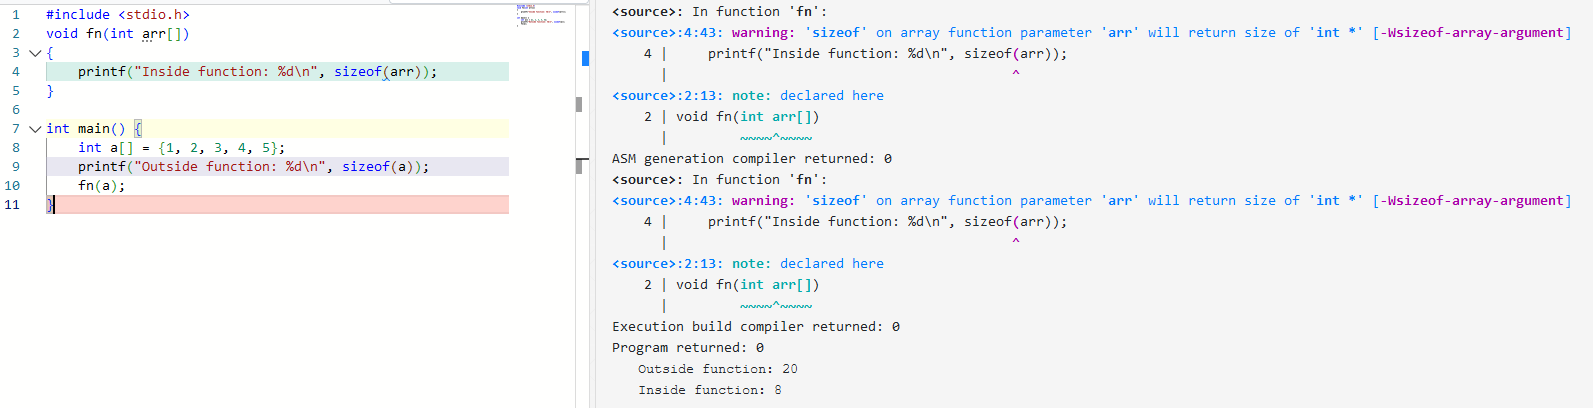
\includegraphics[width=0.99\linewidth]{lekce20/arr_outside_inside.png}
    \end{center}
\end{frame}

\section{Ukazatele (pointery)}

\begin{frame}{Ukazatele (pointery)}
    \begin{block}{Pointer}
        \begin{itemize}
            \item l-values mají místo v paměti
            \item Pomocí operátoru \& lze obdržet adresu proměnné
            \item Tento operátor lze použít jen na l-values!
        \end{itemize}
    \end{block}
    \lstinputlisting[language=C]{lekce20/pointer01.c}
\end{frame}

\begin{frame}{Ukazatele}
    \begin{block}{Dereference}
        \begin{itemize}
            \item Pointer je efektivně proměnná ukazující na oblast adresového prostoru
            \item Typ pointeru nám pak udává na "jak velkou oblast" ukazujeme
            \item Využíváme při interpretaci hodnoty na adrese
            \item Hodnotu uloženou na adrese dostaneme pomocí dereference pointeru
        \end{itemize}
    \end{block}
    \begin{center}
        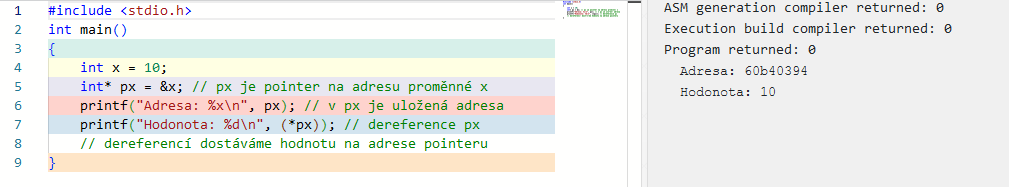
\includegraphics[width=0.99\linewidth]{lekce20/dereference.png}
    \end{center}
\end{frame}

\begin{frame}{Intermezzo: Type casting}
    \begin{block}{Změna typu}
        \begin{itemize}
            \item V některých případech potřebujeme změnit interpretaci (typ) hodnoty uložené v paměti 
            \item Např. dostaneme z nějáké funkce integer a víme že nepřekročí číslo 255, chceme ho tedy převést do charu  \textit{char}
            \item Dělení čísel
        \end{itemize}
    \end{block}
    \lstinputlisting[language=C]{lekce20/cast01.c}
    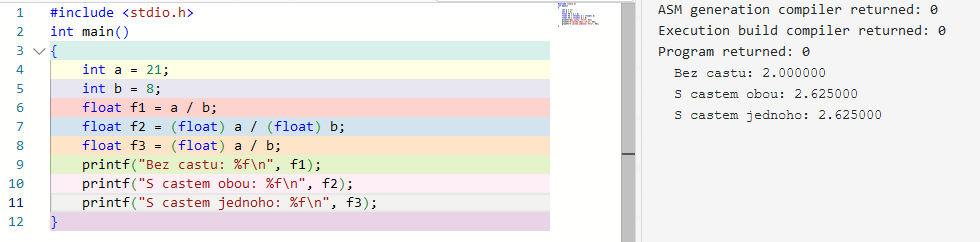
\includegraphics[width=0.87\linewidth]{lekce20/deleni.png}
\end{frame}

\begin{frame}{Intermezzo: Type casting}
    \begin{block}{Cast pointeru}
        \begin{itemize}
            \item Můžeme změnit i typ pointeru
            \item Např. při castu z \textit{int\*} na \textit{char\*} říkáme, že při dereferenci máme s obsahem paměti na dané adrese nakládat jako s charem
        \end{itemize}
    \end{block}
    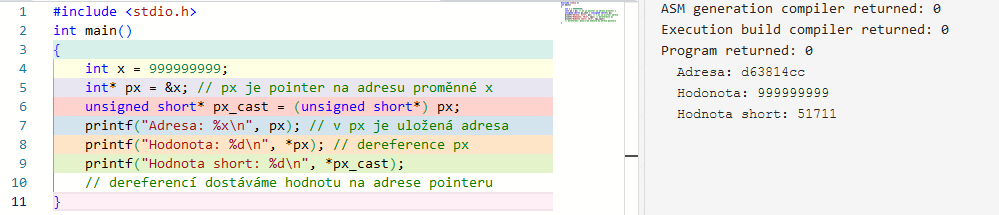
\includegraphics[width=0.99\linewidth]{lekce20/pointer_cast.png}
\end{frame}

\begin{frame}{Intermezzo: Type casting}
    \begin{block}{Implicitní typecast}
        \begin{itemize}
            \item Předchozí ukázky byly explicitní type cast
            \item Často není třeba - implicitní typecast při rozšiřování
        \end{itemize}
    \end{block}
    \lstinputlisting[language=C]{lekce20/cast02.c}
\end{frame}

\begin{frame}{Ukazatele}
        \begin{block}{Volání funkcí - pass by value}
            \begin{itemize}
                \item Při předávání parametru funkci dochází k předání pomocí "pass by value"
                \item Předáváme hodnotu jako r-value (v lokálním scope funkce vytváříme kopii dat které do ní přichází jako parametry)
            \end{itemize}
        \end{block}
        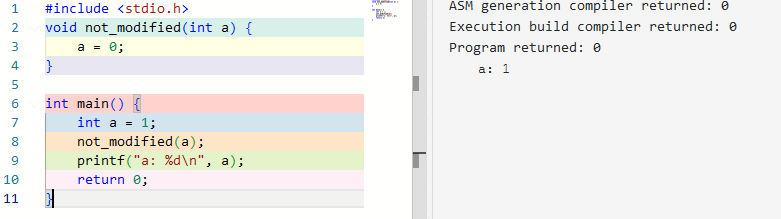
\includegraphics[width=0.99\linewidth]{lekce20/pass_by_value.png}
        \pause
        \begin{block}{Modifikace z funkce}
            \begin{itemize}
                \item Jak vyřešit když potřebujeme modifikovat vnější data uvnitř funkce?
            \end{itemize}
        \end{block}
\end{frame}

\begin{frame}{Ukazatele}
    \begin{block}{Modifikace z funkce}
        \begin{itemize}
            \item Funkcionální přístup - všechny funkce budou \textit{pure} (problém při velkém objemu dat)
            \item Globální scope - modifikované proměnné budou žít v globálním scope (problém s nepřehledností kódu, modifikovatelný globální stav ve větších programech přináší problémy)
            \item Využijeme pointery!
        \end{itemize}
    \end{block}
    \pause
    \begin{block}{Přiřazení dereferencovanému pointeru}
        \begin{itemize}
            \item Dereference pointeru může být i na levé straně přiřazení!
        \end{itemize}
    \end{block}
    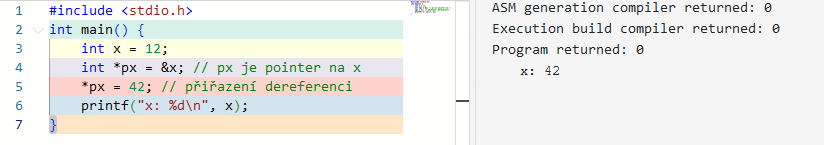
\includegraphics[width=0.99\linewidth]{lekce20/dereference_assignment.png}
\end{frame}

\begin{frame}{Ukazatele}
    \begin{block}{Modifikace z funkce}
        \begin{itemize}
            \item Místo hodnoty bude argumentem funkce pointer na danou hodnotu
            \item Hodnotu dostaneme dereferencí
            \item Hodnotu upravíme přiřazením dereferenci
        \end{itemize}
    \end{block}
    \lstinputlisting[language=C]{lekce20/dereference_assignment01.c}
\end{frame}

\begin{frame}{Konstantní hodnoty}
    \begin{block}{Konstanta}
        \begin{itemize}
            \item Konstanta je hodnota která se za běhu programu nikdy nezmění
            \item Deklarujeme pomocí klíčového slova \textit{const}
        \end{itemize}
    \end{block}
    \lstinputlisting[language=C]{lekce21/const.c}
    \pause
    \begin{block}{Pointer na const}
        \begin{itemize}
            \item Musíme deklarovat že je pointer na konstantu!
            \item Jinak může dojít k přepsání konstanty (!)
        \end{itemize}
    \end{block}
    \lstinputlisting[language=C]{lekce21/const_ptr.c}
\end{frame}

\begin{frame}{Konstantní hodnoty}
    \begin{block}{Pointer na const}
        \begin{itemize}
            \item \textit{const int * identifier} deklaruje pointer na konstantní část paměti
            \item Lze použít i pro "zakázání" mutability uvnitř funkce!
        \end{itemize}
    \end{block}
    \lstinputlisting[language=C]{lekce21/const_func.c}
\end{frame}

\begin{frame}{Konstantní hodnoty}
    \begin{block}{Konstantní pointer}
        \begin{itemize}
            \item Pointer je také proměnná, která se může reassignovat!
            \item Můžeme deklarovat konstantní pointer - klíčové slovo const až za "*"
            \item \textit{const int *} čteme jako "pointer na konstantní int"
            \item \textit{int * const} čteme jako "konstantní pointer na int"
            \item Vše před hvězdičkou udává na jaký typ ukazujeme
        \end{itemize}
    \end{block}
    \lstinputlisting[language=C]{lekce21/const_ptr2.c}
\end{frame}

\begin{frame}{Pole jako ukazatel}
    \begin{block}{Pointer vs array}
        \begin{itemize}
            \item Pointer je ukazatel na lokaci v paměti + informaci o datech uložených
            \item Těchto dat ale může být několik za sebou!
            \item Array je technicky ukazatel na první prvek v paměti (+ informace o celkové velikosti - sizeof)
            \item Array je \textit{const} - hodnotu ukazatele \textbf{nelze} měnit (nelze "pohnout" s adresou)
            \item Array v hlavičce funkce je ale jen pointer, array také můžeme přiřazením převést na pointer
        \end{itemize}
    \end{block}
\end{frame}

\begin{frame}{Aritmetika pointerů}
    \begin{block}{Inkrementace a dekrementace pointerů}
         \begin{itemize}
            \item Nekonstantní pointer může měnit hodnotu
            \item Přičtením/odečtením měníme adresu na kterou ukazujeme
            \item Posouváme se v paměti o délku typu na který pointer ukazuje
         \end{itemize}
    \end{block}
\end{frame}

\begin{frame}{Aritmetika pointerů}
    \begin{block}{Increment int pointer}
        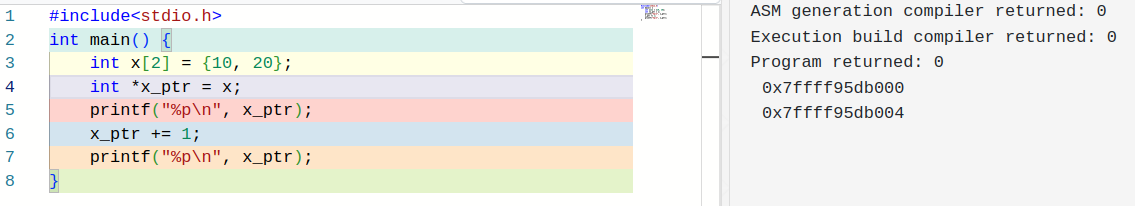
\includegraphics[width=0.95\linewidth]{lekce21/int_ptr_increment.png}
    \end{block}
    \begin{block}{Increment long pointer}
        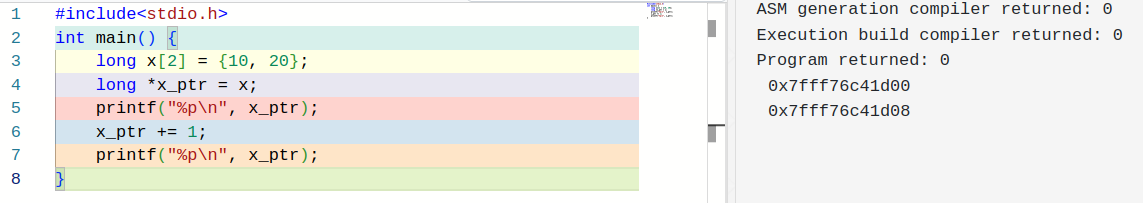
\includegraphics[width=0.95\linewidth]{lekce21/long_ptr_increment.png}
    \end{block}
    \pause
    Adresa se změnila vždy o délku (sizeof) typu!
\end{frame}

\begin{frame}{Intermezzo: Post/Pre increment/decrement}
    \begin{block}{Pre-increment/decrement}
        \begin{itemize}
            \item Provede úpravu dat v paměti (přičtení/odečtení 1)
            \item Poté vrátí již upravenou hodnotu
            \item \textit{++identifier} / \textit{-\,-identifier}
        \end{itemize}
    \end{block}
    \begin{block}{Post-increment/decrement}
        \begin{itemize}
            \item Nejprve se vyhodnotí jako momentální hodnota v paměti
            \item Poté se provede úprava dat v paměti (přištení/odečtení 1)
            \item \textit(identifier++) / \textit{identifier-\,-}
        \end{itemize}
    \end{block}
    \lstinputlisting[language=C]{lekce21/pre_post_increment.c}
\end{frame}

\begin{frame}{Aritmetika pointerů}
    \begin{block}{Porovnávání pointerů}
        \begin{itemize}
            \item Pointery můžeme také porovnávat - má smysl při práci
            s jednou oblastí paměti (bounds checking)
        \end{itemize}
    \end{block}
\end{frame}

\begin{frame}{Aritmetika pointerů}
    \lstinputlisting[language=C]{lekce21/ptr_arithmetics.c}
\end{frame}

\begin{frame}{Textová data}
    \begin{block}{C String}
        \begin{itemize}
            \item Pro textová data se v C používá primárně \textit{char} typ
            \item \textit{char} obsahuje jeden znak (ASCII) - "něco jako 1-String"
            \item Textový řetězec je reprezentován typem \textit{char array}, resp. \textit{char *}
            \item Jak program pozná kde string končí? Musíme předávat parametr o délce?
            \pause
            \item Každý C String je ukončen speciálním znakem s ASCII hodnotou 0.
            \item \textit{Null-terminated byte string}
            \item Když má tedy C string 6 znaků, v paměti je vyhrazena oblast o 1 větší!
        \end{itemize}
    \end{block}
    \lstinputlisting[language=C]{lekce21/c_strings.c}
\end{frame}

\begin{frame}{Textová data}
    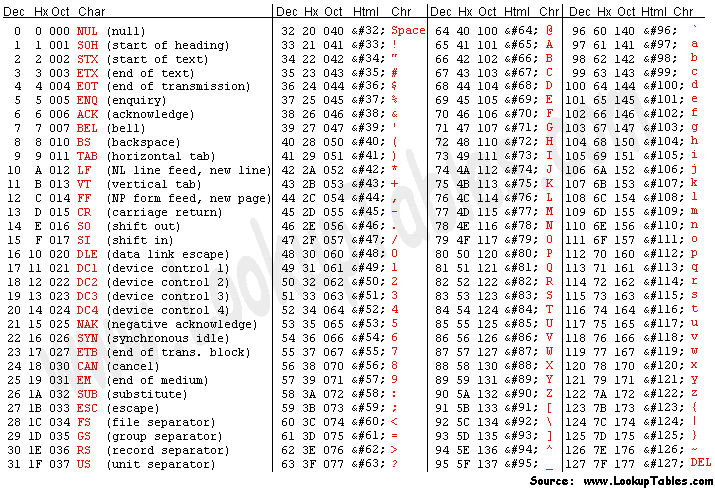
\includegraphics[width=0.95\linewidth]{lekce21/asciifull.png}
\end{frame}

\begin{frame}{Textová data}
    \begin{block}{Funkce pro práci se stringy}
        \begin{itemize}
            \item V různých knihovnách
            \item Include hlavičky - 
            \textit{string.h},
            \textit{stdlib.h},
            \textit{ctype.h} a další
            \item \href{https://en.cppreference.com/w/c/string/byte}{Seznam C-String funkcí}
        \end{itemize}
    \end{block}
    \begin{block}{strlen}
        \begin{itemize}
            \item Jedna z nejdůležitejších funkcí pro práci se stringy - udává
            počet znaků ve stringu (čte string než narazí na null char)
        \end{itemize}
    \end{block}
    \begin{block}{strcmp}
        \begin{itemize}
            \item Porovnávání 2 stringů
            \item Nelze jen porovnat proměnné! Jsou to pointery!
            \item \textit{DEMO - string\_cmp\_wrong.c}
            \item Musí se porovnat charakter po charakteru (to dělá strcmp)
            \item Výjimky pro compile-time známé stringy (optimalizace)
        \end{itemize}
    \end{block}
\end{frame}

\section{Struktury}

\begin{frame}{Struktury}
    \begin{block}{Skládání dat}
        \begin{itemize}
            \item Nechceme pracovat jen s primitivními daty - přidání struktury
            \item struct type - kompozitní typ, skládá se z několika jednodušších struktur/primitivů
        \end{itemize}
    \end{block}
    \lstinputlisting[language=C]{lekce21/struct.c}
\end{frame}

\begin{frame}{Struktury}
    \begin{block}{Přístup k datům}
        \begin{itemize}
            \item Přímý přístup (pomocí member access operátoru \textit{"."})
            \item Přístup přes pointer (pomocí operátoru \textit{"->"})
        \end{itemize}
    \end{block}
    \lstinputlisting[language=C]{lekce21/struct_access.c}
\end{frame}

\begin{frame}{Struktury}
    \begin{block}{Struct jako argument funkce}
        \begin{itemize}
            \item Parametry se předávají jako \textbf{value}
            \item Při předání struktury přímo se předá její \textbf{kopie}
            \item Pro velké struktury je pass-by-value drahá operace - hodně kopírování
            \item Předávání pointerem - předá se jen ukazatel na to, kde v paměti struktura je
            \item Při předání pointerem můžeme modifikovat
            \item Můžeme opět aplikovat const modifier - nelze pak modifikovat struct memers
        \end{itemize}
    \end{block}
\end{frame}

\begin{frame}{Struktury}
    \lstinputlisting[language=C]{lekce21/struct_passing.c}
\end{frame}

\begin{frame}{Struktury}
    \begin{block}{Inicializační funkce}
        \begin{itemize}
            \item Často se setkáme s použitím inicializačních funkcí
            \item Pomáhají s parametrizací - díky hlavičce funkce lépe vidíme
            co hodnota znamená
        \end{itemize}
    \end{block}
    \lstinputlisting[language=C]{lekce21/struct_constructor.c}
\end{frame}

\begin{frame}{Intermezzo: NULL pointer}
    \begin{block}{NULL}
        \begin{itemize}
            \item Obsažen v standardní knihovně, hodnota ((void*)0)
            \item Neukazuje na žádné místo v paměti!
            \item Používá se jako "speciální hodnota" nebo inicializační hodnota
            \item Garantovaná nerovnost s jakýmkoliv pointerem na proměnnou (nebo funkci)
            \item Dereference NULL pointeru způsobí chybu programu!!!
            \item Velmi častá (a kritická) chyba v C programech
        \end{itemize}
    \end{block}
    \lstinputlisting[language=C]{lekce21/null_ptr.c}
\end{frame}

\begin{frame}{Ukázka - linked list}
    \lstinputlisting[language=C]{lekce21/linked_list.c}
\end{frame}

\begin{frame}{Ukázka - linked list}
    Stále není ideální - musíme explicitně říkat v jakém scope žijí prvky listu tím,
    že je tam deklarujeme - nelze psát \textit{cons(30, cons(20, cons(10, NULL)))}
    \\
    Budeme potřebovat dynamickou alokaci paměti - později
\end{frame}

\begin{frame}{l-value scope}
    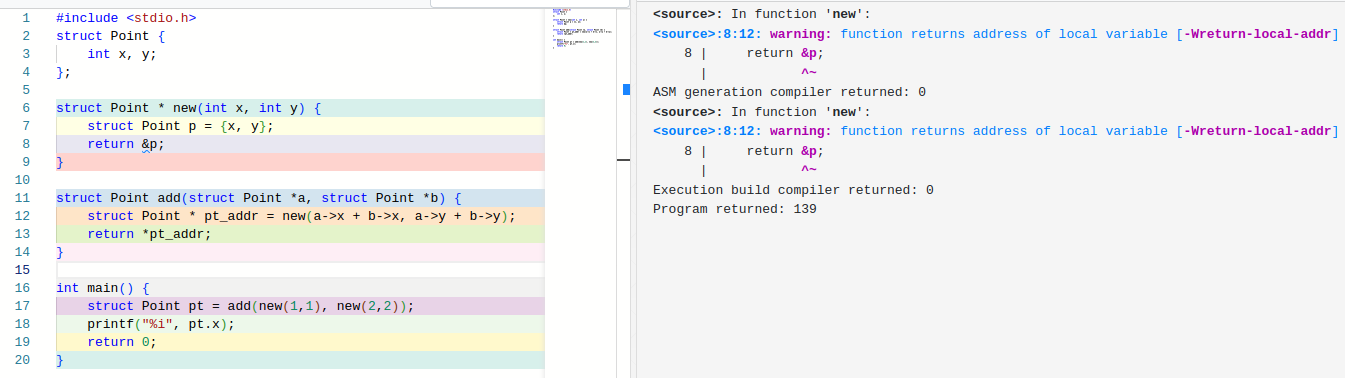
\includegraphics[width=0.99\linewidth]{lekce21/local_variable.png}
\end{frame}

\begin{frame}{Union}
    \begin{block}{Union typy}
        \begin{itemize}
            \item struct slouží jako product type (stejně jako v BSL/ISL),
            kombinuje více hodnot do jednoho typu
            \item V některých případech potřebujeme sum type - předat jednu hodnotu
            nabývající jednoho z více typů (v ISL např. Maybe Number - Number nebo \#f)
            \item union typy - deklarují všechny možnosti, realizuje se pouze jedna
        \end{itemize}
    \end{block}
    \lstinputlisting[language=C]{lekce21/union.c}
\end{frame}

\begin{frame}{Union}
    \begin{block}{Union typy}
        \begin{itemize}
            \item Union typy tedy obsahují pouze jednu z možností (sum type)
            \item Jak poznat kterou? Obalení do struct s tagem udávající možnost
            \item Použití tzv. enum typu pro označení možnosti (tag)
        \end{itemize}
    \end{block}
\end{frame}

\begin{frame}{Enumerace}
    \begin{block}{Enum typy}
        \begin{itemize}
            \item Výčtové typy
            \item Překládají se na integer
            \item Slouží ke zlepšení korektnosti za compile-time
        \end{itemize}
    \end{block}
    \lstinputlisting[language=C]{lekce21/enum.c}
\end{frame}

\begin{frame}{Enumerace}
    \begin{block}{Enum typy}
        \begin{itemize}
            \item Lze explicitně specifikovat jaký integer bude přiřazen
        \end{itemize}
    \end{block}
    \lstinputlisting[language=C]{lekce21/enum_explicit.c}
\end{frame}

\begin{frame}{Tagged union}
    DEMO: tagged\_union.c
\end{frame}

\section{Dynamická alokace paměti}

\begin{frame}{Dynamická alokace}
    TBD
\end{frame}

\end{document}